\chapter{Introduction}
Artificial intelligence is playing more prominent role in our daily lives by demonstrating human intelligence by machines, especially computer systems. The field includes learning, reasoning and self-correction. These can be described as the acquisition of information and rules for using the information, using the rules to reach approximate or definite conclusions. It has become more important to make machines able to communicate through natural language with human or among machines themselves. Learning algorithms for natural language understanding in language translation, reading comprehension have progressed at a rate in recent years that never done before, but that lack ultimate aspects of how humans understand and produce natural language. Mainly humans develop language understanding and producing by being embodied in an environment which they can realize and interact with other humans~\cite{DBLP:journals/corr/abs-1807-03367}.

In many tasks understanding compositional language in context is very complex. Reasoning about sets of objects, quantities, comparisons and spatial relations are required in visual question answering and robot instruction systems. Robust language understanding is required when instructing assembly-line or home assistance robots to manipulate objects in random environments. And this is only partially addressed by existing datasets~\cite{Suhr2017ACO}.

Since the early days of artificial intelligence, the problem of interpreting instructions written in natural language has been widely studied. The automation of tasks that currently require human participation would be enabled by mapping instructions to a sequence of executable actions~\cite{RL}.



``Natural Language" refers to a human language that is used for everyday communication by humans; languages like English, Bengali or Portuguese as distinct from the typically artificial command. Artificial language like programming language and mathematical transcripts, natural languages have evolved over generations, and hard to keep down with explicit rules. NLP based technologies are becoming increasingly widespread. For example, phones and handheld computers support text suggestion and handwriting recognition;web search engines provide access to information locked up in noisy text data;machine translation allows us to recover written texts in different language and read them in another language; text analysis enables us to classify sentiment in different reviews or blogs post. By providing a more natural human-machine interfaces and more sophisticated access to stored data, a central role is played by language processing in multilingual information society~\cite{NLPbook}.

It is straightforward to induce our hands on countless words of text. What will we have a tendency to do with it, forward we are able to write some easy programs? We're all terribly accustomed to text, since we have a tendency to scan and write it on a daily basis. Here we'll treat text as data for the programs we have a tendency to write, programs that manipulate and analyze it in an exceedingly type of attention-grabbing ways.
\section{Robot Navigation}
Navigation refers to the strategy of crucial aspects like position, speed, and direction throughout travel. within the pre-modern era, direction associate degreed position were determined mistreatment an measuring instrument, a compass, and a map; these square measure currently thought of primitive kinds of navigation. As a results of fashionable developments in science and technology, precise positions and speeds square measure determined mistreatment instrumentation like artificial satellites, international navigation satellite system (GNSS), direction systems (INS), etc~\cite{NAV}.

\section{Automatic Natural Language Understanding}
At a strictly sensible level, we tend to all want facilitate to navigate the universe of knowledge fast up in text on the net. Search engines are crucial to the expansion and recognition of the net, however have some shortcomings. It takes talent, knowledge, and a few luck, to extract answers to such queries as: \emph{What tourist sites can I visit between Philadelphia and Pittsburgh on a limited budget?What do experts say about digital SLR cameras? What did the trusted commentators predict about the steel market last week?} Getting a machine to answer them automatically involves a variety of language process tasks, as well as info extraction, inference, and account, and would want to be dispensed on a scale and with grade of hardiness that's still on the far side our current capabilities.

On a a lot of philosophical level, a long-standing challenge at intervals AI has been to create intelligent machines, and a serious a part of intelligent behavior is knowing language. for several years this goal has been seen as too troublesome. However, as information science technologies become a lot of mature, and sturdy strategies for analyzing unrestricted text become a lot of widespread, the prospect of language understanding has re-emerged as a plausible goal~\cite{NLPbook}.

In this section we tend to describe some language understanding technologies, to allow a way of the attention-grabbing challenges that area unit associated with NLP.
\subsection{Word Sense Disambiguation:}
In word meaning disambiguation we wish to figure out that sense of a word was supposed in an exceedingly given context. Contemplate the ambiguous words serve and dish:

\begin{enumerate}[a.]
    \item serve: help with lunch or drink; hold an office; put football into play
    \item dish: glass; course of a meal; communications devices    
\end{enumerate}
In a sentence containing the phrase: he served the dish, square measure able to notice that each serve and dish are being employed with their food meanings. It's unlikely that the subject of dialogue shifted from sports to crockery within the space of 3 words. This might force us to create outre pictures, sort of a professional tennis player removing his or her frustrations on a china tea-set arranged out beside the court. In alternative words, we have a tendency to automatically clear up words exploitation context, exploiting the straightforward incontrovertible fact that close words have closely connected meanings. As another example of this discourse result, take into account the word by, that has many meanings, e.g.: the book by Russel (agentive -- Russel was the author of the book); the match by the stove (locative -- the stove is where the match is); and submit by Saturday (temporal -- Saturday is the time of the submission). Observe in (c) that the meaning of the italicized word helps us interpret the meaning of by.

\begin{enumerate}[a.]
    \item The lost women were found by the searchers (agentive)
    \item The lost women were found by the mountain (locative)
    \item The lost women were found by the afternoon (temporal)    
\end{enumerate}

\subsection{Pronoun Resolution}
A deeper reasonably language understanding is to figure out "who did what to whom" — i.e., to observe the subjects and objects of verbs. You learnt to try and do this in grammar school, however it's tougher than you may assume. In the sentence the thieves stole the paintings it's simple to detect who performed the stealing action. Consider 3 doable following sentences in (c), and check out to see what was sold, caught, and found (one case is ambiguous).
\begin{enumerate}[a.]
    \item The thieves stole the paintings. They were subsequently sold.
    \item The thieves stole the paintings. They were subsequently caught.
    \item The thieves stole the paintings. They were subsequently found.
\end{enumerate}
Answering this question involves looking for the preposition of the pronoun they, either thieves or paintings. One of the calculation techniques to address this problem includes anaphora resolution -- identifying what a pronoun or noun phrase means -- and labeling semantic role -- identifying the relation between a noun phrase and the verb (as agent, patient, instrument, and so on).

\subsection{Generating Language Output}
If we are able to automatically solve such issues of language understanding, we are going to solve the tasks that involve generating language output, like responding to a question and translating language from one form to another. In the initial case, a machine ought to be ready to answer a user's query regarding to text collection.

\begin{enumerate}[a.]
    \item Text: ... The thieves stole the paintings. They were subsequently sold. ...
    \item Human: Who or what was sold?
    \item Machine: The paintings.
\end{enumerate}
The answer of machine proves that it has correctly worked out that \emph{they} doesn't refer to the thieves but to paintings. 

\subsection{Spoken Dialog Systems}
In the study of past of artificial intelligence, the main measure of intelligence has been a linguistic, Turing test: if a dialog system, responding to a user's text input, can perform so naturally that we can't differentiate it from human-generated reactions. Can't i? On the contrary, today's commercial dialog systems are very limited but still perform useful functions in short-term domains, as we can see here:\\
S: How may I help you?\\
U: Deliver some food from the list to Shahidullah Hall after buying these from TSC.\\
S: Buying food from TSC first and then deliver these to Shahidullah Hall?\\
U: Yes.\\

We could not ask the machine to produce driving directions or details of nearby restaurants unless the specified info had already been hold on and appropriate question-answer pairs had been incorporated into the language processing system.

Observe that this system understands the sequence of working plan based on the instruction: the user tells an instruction in complex way and the system correctly determines from this that the user wants to deliver some food but it needs to buy these foods first. This assumption seems so obvious that you probably didn't notice that it was trained, yet a natural language system needs to be completed with this skill to communicate naturally. WIthout it, when asked \emph{Deliver some food from the list to Shahidullah Hall after buying these from TSC.}, a system might plan to deliver first and to buy food from TSC.
Usually contextual assumptions and business logic is used in commercial dialogue systems to ensure that a user can request or provide information that pays for specific applications.

\begin{figure}
    \centering
    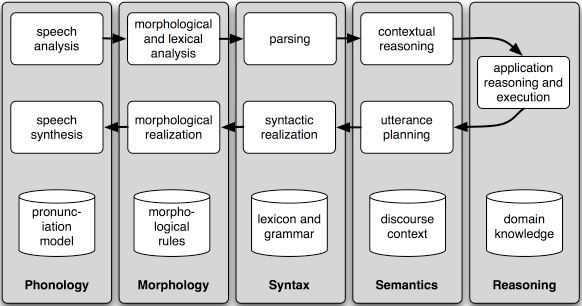
\includegraphics[width=1\textwidth]{pipline}
    \caption{Simple Pipeline Architecture for a Spoken Dialogue System\cite{NLPbook}}
    \label{fig:1}
\end{figure}

In Figure~\ref{fig:1}, \emph{Spoken signal (top left) is taken, speech is recognized, words are parsed and taken in context, application-specific actions occur (top right); a reaction is planned, is realized as a syntactic structure, then to the words that are properly replaced and finally to the spoken output; The different types of linguistic knowledge inform each level of the process.}

Dialogue systems give us the fundamental pipeline for NLP. Figure~\ref{fig:1} 
shows the architecture of a normal dialog system. One of the few language-understanding elements that move left to right at the top of the diagram is "Pipeline". This map is a kind of money-making from the spicinput through the syntactic parsing. In the middle, the opposite pipeline of elements to convert the concept from right to left. These elements create dynamic aspects of the system. Below the diagram there are a few representative organizations of static information: the collection of language-related data for processing materials to do their job.

\subsection{Information Extraction}
With rise of digital age, there's associate degree explosion of data within the sort of news, articles, blogs, social media, and so on. A lot of of this knowledge lies in unstructured type and manually managing and effectively creating use of it's tedious, boring and labor intensive. This explosion info of data of knowledge and want for a lot of subtle and economical information handling tools provides rise to data Extraction(IE) and knowledge Retrieval(IR) technology. data Extraction systems takes linguistic communication text as input and produces structured data mere by bound criteria, that's relevant to a selected application. numerous sub-tasks of i.e. like Named Entity Recognition, grammatical relation Resolution, Named Entity Linking, Relation Extraction, mental object reasoning forms the building blocks of assorted high finish linguistic communication process (NLP) tasks like MT, Question-Answering System, linguistic communication Understanding, Text summarisation and Digital Assistants like Siri, Cortana and Google Now~\cite{DBLP:journals/corr/abs-1807-02383}.
\begin{figure}[htbp]
    \centering
    \includegraphics[width=.8\textwidth]{ie}
    \caption{Simple Pipeline Architecture for an Information Extraction System~\cite{DBLP:journals/corr/abs-1807-02383}.}
    \label{fig:2}
\end{figure}

Figure~\ref{fig:2}shows the design for a straightforward info extraction system. It begins by process a document victimization many of the procedures: 1st, the raw text of the document is split into sentences employing a sentence segmenter, and every sentence is any divided into words employing a tokenizer. Next, every sentence is labeled with part-of-speech tags, which can prove terribly useful within the next step, named entity detection. during this step, we tend to look for mentions of probably attention-grabbing entities in every sentence. Finally, we tend to use relation detection to look for doubtless relations between completely different entities within the text.
\section{Task Definition}
In our project, we are developing an agent that will follow Bengali instructions to navigate in real-life visual environment.
\begin{itemize}
	\item Inputs: Text based instructions in Bengali language.
	\item Outputs: Mapping instructions and visual observations to actions and execute them in the environment.
\end{itemize}

\section{Motivation}
Computers are good at operating with structured information like spreadsheets and info tables. However we humans typically communicate in words, not in tables. That’s unfortunate for computers. Loads of data within the world is unstructured raw text in English or another human language. however will we have a tendency to get a pc to know unstructured text and extract information from it?
Advances in AI are sanctioning increasingly more refined, capable technologies to achieve massive client populations. Such systems provide unprecedented potential for AI to assist in a very type of human-centric applications like elder care and home maintenance. However, natural, easy-touse interfaces to such systems, like those using linguistic communication, square measure insulation behind. As robots become additional prevalent—and because the would like for the services they will provide grows—the importance of permitting non-expert users to act with them naturally and well will increase. linguistic communication is a superb modality for finish users to offer directions and teach robots concerning their environments~\cite{ijcai2018-810}. 

As long as computers are around, programmers are attempting to write down programs that perceive languages like English. the rationale is pretty obvious humans are writing things down for thousands of years and it'd be extremely useful if a laptop might scan and perceive all that knowledge.
NLP is very important for scientific, economic, social, and cultural reasons. NLP is experiencing rapid climb as its theories and strategies square measure deployed in a very style of new language technologies. For this reason it's necessary for a good vary of individuals to possess a operating data of NLP. among business, this includes folks in human-computer interaction, business data analysis, and internet software system development. among academe, it includes folks in areas from humanities computing and corpus linguistics through to engineering and computing~\cite{NLPbook}.
\newpage
\section{Objectives}
By developing the project, we will learn:
\begin{itemize}
    \item To manipulate large corpora, explore linguistic models and analyze language data.
    \item To use the key concepts from NLP and linguistics to describe and analyse language.
    \item To use data structures and linguistics algorithms in robust language processing software.
    \item To extract knowledge from natural language.
    \item To map instructions from natural language to actions.
    \item To deploy an intelligent agent to execute actions in a particular visual environment.
\end{itemize}





